% Options for packages loaded elsewhere
\PassOptionsToPackage{unicode}{hyperref}
\PassOptionsToPackage{hyphens}{url}
\PassOptionsToPackage{dvipsnames,svgnames,x11names}{xcolor}
%
\documentclass[
  twocolumn]{article}

\usepackage{amsmath,amssymb}
\usepackage{setspace}
\usepackage{iftex}
\ifPDFTeX
  \usepackage[T1]{fontenc}
  \usepackage[utf8]{inputenc}
  \usepackage{textcomp} % provide euro and other symbols
\else % if luatex or xetex
  \usepackage{unicode-math}
  \defaultfontfeatures{Scale=MatchLowercase}
  \defaultfontfeatures[\rmfamily]{Ligatures=TeX,Scale=1}
\fi
\usepackage{lmodern}
\ifPDFTeX\else  
    % xetex/luatex font selection
\fi
% Use upquote if available, for straight quotes in verbatim environments
\IfFileExists{upquote.sty}{\usepackage{upquote}}{}
\IfFileExists{microtype.sty}{% use microtype if available
  \usepackage[]{microtype}
  \UseMicrotypeSet[protrusion]{basicmath} % disable protrusion for tt fonts
}{}
\makeatletter
\@ifundefined{KOMAClassName}{% if non-KOMA class
  \IfFileExists{parskip.sty}{%
    \usepackage{parskip}
  }{% else
    \setlength{\parindent}{0pt}
    \setlength{\parskip}{6pt plus 2pt minus 1pt}}
}{% if KOMA class
  \KOMAoptions{parskip=half}}
\makeatother
\usepackage{xcolor}
\usepackage[left=1cm, right=1cm, top=1.5cm, bottom=1.5cm]{geometry}
\setlength{\emergencystretch}{3em} % prevent overfull lines
\setcounter{secnumdepth}{-\maxdimen} % remove section numbering
% Make \paragraph and \subparagraph free-standing
\ifx\paragraph\undefined\else
  \let\oldparagraph\paragraph
  \renewcommand{\paragraph}[1]{\oldparagraph{#1}\mbox{}}
\fi
\ifx\subparagraph\undefined\else
  \let\oldsubparagraph\subparagraph
  \renewcommand{\subparagraph}[1]{\oldsubparagraph{#1}\mbox{}}
\fi


\providecommand{\tightlist}{%
  \setlength{\itemsep}{0pt}\setlength{\parskip}{0pt}}\usepackage{longtable,booktabs,array}
\usepackage{calc} % for calculating minipage widths
% Correct order of tables after \paragraph or \subparagraph
\usepackage{etoolbox}
\makeatletter
\patchcmd\longtable{\par}{\if@noskipsec\mbox{}\fi\par}{}{}
\makeatother
% Allow footnotes in longtable head/foot
\IfFileExists{footnotehyper.sty}{\usepackage{footnotehyper}}{\usepackage{footnote}}
\makesavenoteenv{longtable}
\usepackage{graphicx}
\makeatletter
\def\maxwidth{\ifdim\Gin@nat@width>\linewidth\linewidth\else\Gin@nat@width\fi}
\def\maxheight{\ifdim\Gin@nat@height>\textheight\textheight\else\Gin@nat@height\fi}
\makeatother
% Scale images if necessary, so that they will not overflow the page
% margins by default, and it is still possible to overwrite the defaults
% using explicit options in \includegraphics[width, height, ...]{}
\setkeys{Gin}{width=\maxwidth,height=\maxheight,keepaspectratio}
% Set default figure placement to htbp
\makeatletter
\def\fps@figure{htbp}
\makeatother

\usepackage{xcolor}
\usepackage{titlesec}
\definecolor{royalblue}{RGB}{65, 105, 225}
\titleformat{\section}{\normalfont\Large\bfseries\color{royalblue}}{}{0pt}{}
\titleformat{\subsection}{\normalfont\large\bfseries\color{royalblue}}{}{0pt}{}
\makeatletter
\@ifpackageloaded{caption}{}{\usepackage{caption}}
\AtBeginDocument{%
\ifdefined\contentsname
  \renewcommand*\contentsname{Table of contents}
\else
  \newcommand\contentsname{Table of contents}
\fi
\ifdefined\listfigurename
  \renewcommand*\listfigurename{List of Figures}
\else
  \newcommand\listfigurename{List of Figures}
\fi
\ifdefined\listtablename
  \renewcommand*\listtablename{List of Tables}
\else
  \newcommand\listtablename{List of Tables}
\fi
\ifdefined\figurename
  \renewcommand*\figurename{Figure}
\else
  \newcommand\figurename{Figure}
\fi
\ifdefined\tablename
  \renewcommand*\tablename{Table}
\else
  \newcommand\tablename{Table}
\fi
}
\@ifpackageloaded{float}{}{\usepackage{float}}
\floatstyle{ruled}
\@ifundefined{c@chapter}{\newfloat{codelisting}{h}{lop}}{\newfloat{codelisting}{h}{lop}[chapter]}
\floatname{codelisting}{Listing}
\newcommand*\listoflistings{\listof{codelisting}{List of Listings}}
\makeatother
\makeatletter
\makeatother
\makeatletter
\@ifpackageloaded{caption}{}{\usepackage{caption}}
\@ifpackageloaded{subcaption}{}{\usepackage{subcaption}}
\makeatother
\ifLuaTeX
  \usepackage{selnolig}  % disable illegal ligatures
\fi
\usepackage{bookmark}

\IfFileExists{xurl.sty}{\usepackage{xurl}}{} % add URL line breaks if available
\urlstyle{same} % disable monospaced font for URLs
\hypersetup{
  colorlinks=true,
  linkcolor={blue},
  filecolor={Maroon},
  citecolor={Blue},
  urlcolor={Blue},
  pdfcreator={LaTeX via pandoc}}

\author{}
\date{}

\begin{document}

\setstretch{1.1}
\twocolumn[{
\begin{center}
\textbf{\textcolor{royalblue}{\Large Predicting House Prices Using Key Property Features Through Multiple Regression}}
\end{center}

\vspace{0.2cm}

\begin{center}
\textit{Hamza Ahmed, Cifti Saggu, Daniella Jaqin, Mike Xu, Zichen Liu}
\end{center}
\vspace{1cm}
}]

\section{Abstract}\label{abstract}

This report examines key variables influencing house prices in New York,
focusing on the relationships between property characteristics and
pricing to provide insights for stakeholders in the real estate market.
Using multiple regression analysis, we found that the number of
bathrooms and rooms have the most significant positive impact on housing
prices, reflecting the value buyers place on space and amenities in a
densely populated city like New York. Additionally, the age of a house
negatively impacts its price, indicating a preference among buyers for
newer properties.The model's performance indicators, including MAE and
RMSE, suggest reliable accuracy in estimating price fluctuations.
Additionally, consistent AIC and BIC values indicate a good balance
between accuracy and simplicity for our selected model. This report
serves as a useful reference for property valuation and supports
stakeholders in making informed decisions.

\section{Introduction}\label{introduction}

The current housing market is a complex and dynamic environment
influenced by various factors. Being able to understand the key drivers
of house prices is crucial for stakeholders, including potential buyers,
sellers, and investors. This analysis aims to answer several important
questions. These questions are: What property features most
significantly impact house prices? How do these features interact with
one another to influence overall value? By utilising multiple regression
analysis, we seek to quantify the relationships between key numeric
variables and house prices, providing insights that can guide
decision-making in the real estate market.

\section{Data set}\label{data-set}

The dataset used for this analysis was collected from The Data And Story
Library (DASL), capturing a range of properties across New York. It
includes numerous variables related to property characteristics,
focusing on numeric predictors that correlate well with regression
analysis. The key variables in this dataset include Lot Size, Age, Land
Value, Living Area, Pct College, Bedrooms, Bathrooms, and Rooms. The
dataset excludes categorical variables, focusing on continuous numeric
features that provide measurable attributes relevant to property
valuation. This approach enables a clearer analysis of how these
features affect house prices, allowing for a more systematic
understanding of their impacts.

\section{Analysis}\label{analysis}

To analyse the dataset using multiple regression, we focused on the
numeric predictor variables, specifically Lot Size, Age, Land Value,
Living Area, Pct College, Bedrooms, Bathrooms, and Rooms. We chose to
exclude categorical variables, as many such as waterfront or fireplaces
are based on personal house preferences rather than common, quantifiable
features that may have a consistent impact on price. Continuous numeric
features further provide measurable attributes that are easier to
evaluate a prediction of price.

To ensure the model's validity, the numeric predictors were
systematically checked against the key multiple regression assumptions.
For linearity, we visualized each predictor's relationship with
log-transformed price, leading to the log-transformation of age due to
slight curvature. \textbf{(Appendix 1)} Independence was verified by
assessing the Variance Inflation Factor (VIF) values, where all values
were below 5, indicating acceptable levels of multicollinearity
\textbf{( Appendix 2)}. Homoskedasticity was examined through a residual
plot \textbf{(Appendix 3)}, suggesting constant variance of residuals.
Normality was checked with a Q-Q plot \textbf{(Appendix 4)}, which
showed residuals following the quantile line closely, with minor
deviations at the tails. Based on these checks, we confirmed that the
final model meets the assumptions required for multiple regression
without further adjustments.

\section{Results}\label{results}

For our results, we evaluated three model selection methods, the forward
selection, backward selection, and exhaustive search. Interestingly, all
three models produced identical performance metrics \textbf{(RMSE:
0.2686, MAE: 0.2042, R²: 0.5613)} and shared the same \textbf{AIC
(451.24)} and \textbf{BIC (483.64)} values. Since the statistical
criteria did not differentiate them, we selected the forward model for
its practical advantages.Forward selection is computationally efficient
compared to exhaustive search, which becomes costly with additions to
the dataset. While less expensive than exhaustive search, backward
selection can still retain interdependent or spurious variables, raising
the risk of overfitting. The forward model avoids these issues by adding
only essential variables, resulting in a more robust and interpretable
model that mirrors real-world property evaluation. Its gradual selection
approach also builds stakeholder confidence by focusing on factors
typically prioritised in property assessments making forward selection a
practical, reliable choice.

Our final model for predicting house prices is given by the equation:

\(\textcolor{teal}{\log(\text{Price})} = \textcolor{teal}{11.395433} + \textcolor{teal}{0.000377} \times \textcolor{teal}{\text{Living Area}} + \textcolor{teal}{0.103651} \times \textcolor{teal}{\text{Bathrooms}} - \textcolor{teal}{0.047154} \times \textcolor{teal}{\log(\text{Age})} + \textcolor{teal}{0.007997} \times \textcolor{teal}{\text{Rooms}}\)

This equation shows how each predictor contributes to house price, both
statistically and practically. Adding a bathroom or a room results in
about a 10.37\% and 0.8\% price increase, respectively, due to the
significance of each ``unit increase.'' In real terms, an additional
bathroom or room is a substantial change, aligning with how buyers
perceive these features in property value. Living area, with a smaller
coefficient (0.0004), can still impact price substantially but with a
larger `unit size' (e.g., 1,000 square feet). The negative coefficient
for age (-0.0472) reflects a preference for newer homes among
stakeholders. This interpretation balances statistical results with
real-world relevance, ensuring our insights are meaningful for
stakeholders.

\section{Discussion}\label{discussion}

Our analysis uses a multiple regression model to examine key property
characteristics that influence New York home prices, focusing on numeric
predictor variables.

-Appendix 1 shows the linear relationship between the log-converted
price and the predictors (log age, living area, rooms and bathrooms),
confirming the correlation of the predictors.

-In Appendix 2, VIF values verify independence, and all values are below
5.

- The residuals plot in Appendix 3 shows that the variance of the
residuals is constant.

- The Q-Q chart in Appendix 4 shows that residuals follow a normal
distribution. Our final model provides a look at how certain variables
(living area, number of bathrooms, rooms, and age) affect house prices:

- Although the coefficient for living area is small (0.0004), it doesn't
fully capture the value buyers place on space as large living areas
(e.g.1,000 square feet) reflect a substantial relative impact on price.
Each additional bathroom raises the price by approximately 10.37\%,
highlighting the high value buyers place on space and amenities

- Age has a negative coefficient, indicating that as homes age, their
value generally declines.

- The increase in the number of rooms resulted in a small increase in
prices (0.8\%). These findings have benefits for stakeholders, including
potential future homeowners, investors and policymakers, who rely on
this knowledge to make decisions.

\section{Limitations and Future
Improvements}\label{limitations-and-future-improvements}

Our dataset presented limitations due to its predominantly categorical
nature, which restricted the continuous predictors available for
modeling. Of the 17 initial variables, only 6 continuous ones met the
assumptions for regression, reducing the model's depth and limiting its
ability to capture finer details. To enhance our model, future work
could benefit from a more comprehensive dataset that includes
location-specific and economic indicators, such as inflation and
interest rates, as well as additional continuous predictors for greater
granularity.

Real estate prices often exhibit non-linear trends that cannot be fully
captured by a linear model like multiple regression, limiting the range
of housing features our model can analyze. Exploring non-linear models,
such as decision trees or random forests, could better accommodate
categorical and non-linear variables, allowing for more complex
relationships that a linear model cannot capture. Finally, since the
model is specific to New York, its application to other regions or
markets is limited, suggesting that further region-specific models may
be required

\section{Conclusion}\label{conclusion}

In summary, the regression model we used in this report identifies the
key variables that influence New York house prices, providing a useful
tool for property valuation. Hopefully, our findings can provide
meaningful insights to those involved in the housing market that can
help them make informed decisions.

\subsection{Git Repository}\label{git-repository}

https://github.sydney.edu.au/djaq0514/L12G03

\newpage

\subsection{Appendix 1}\label{appendix-1}

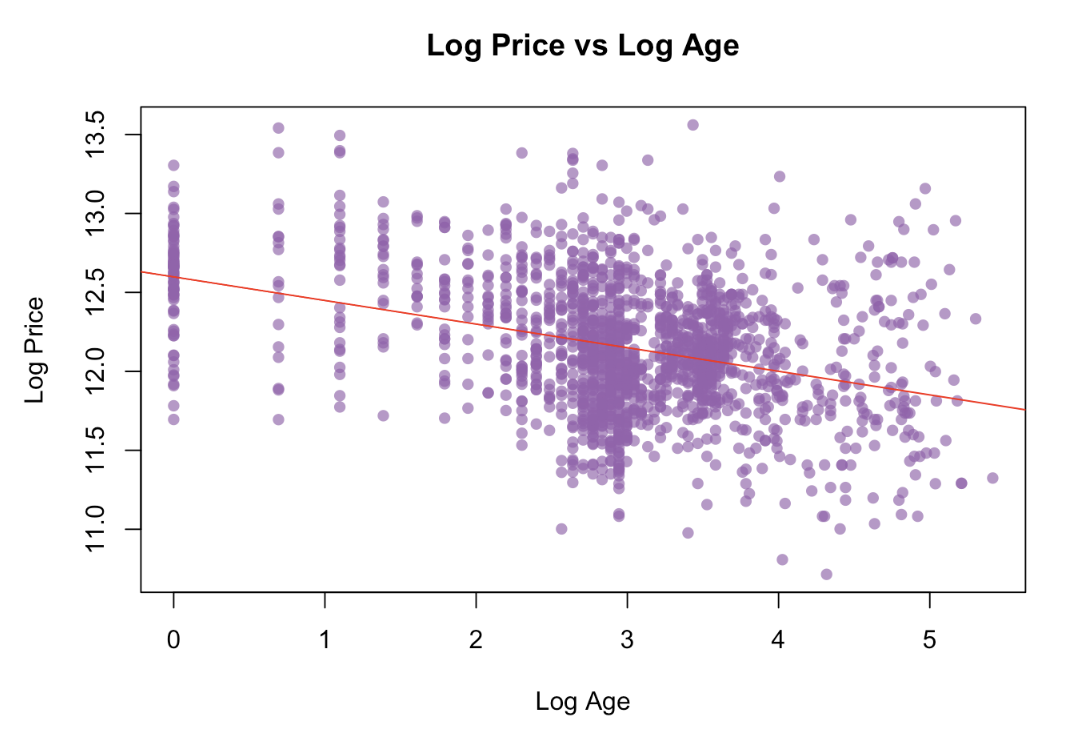
\includegraphics[width=0.43\textwidth,height=\textheight]{A1 log age.png}
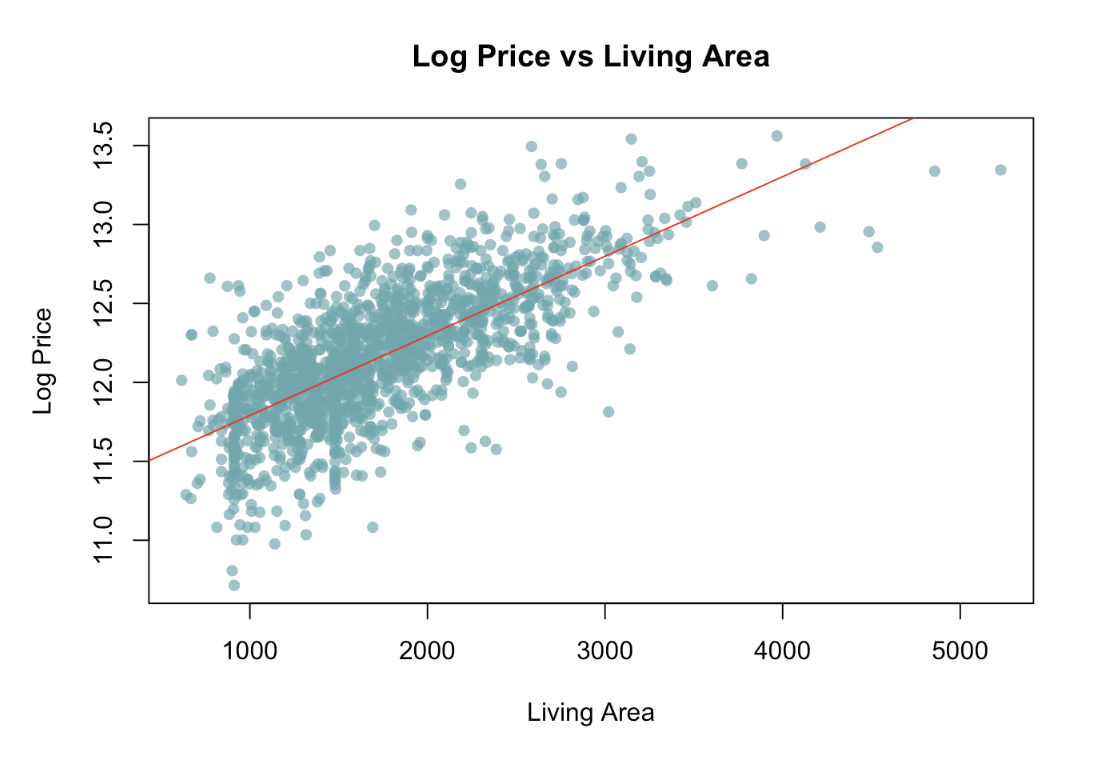
\includegraphics[width=0.43\textwidth,height=\textheight]{A1 Living Area.png}
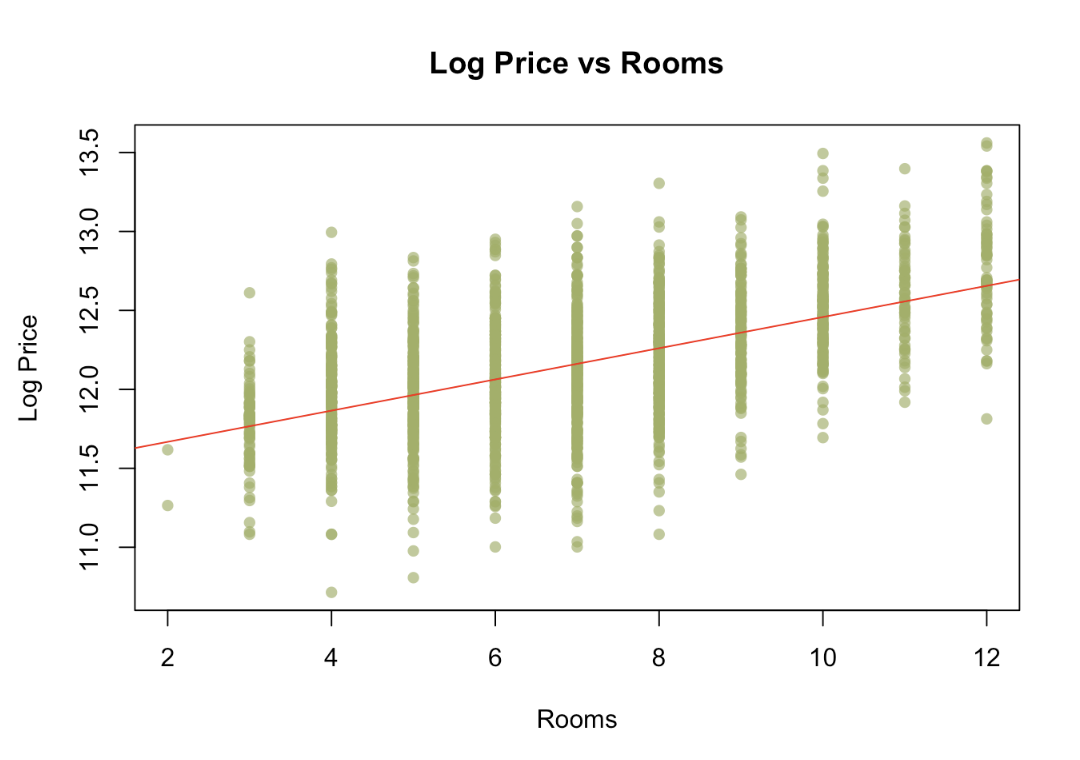
\includegraphics[width=0.43\textwidth,height=\textheight]{A1 Rooms.png}
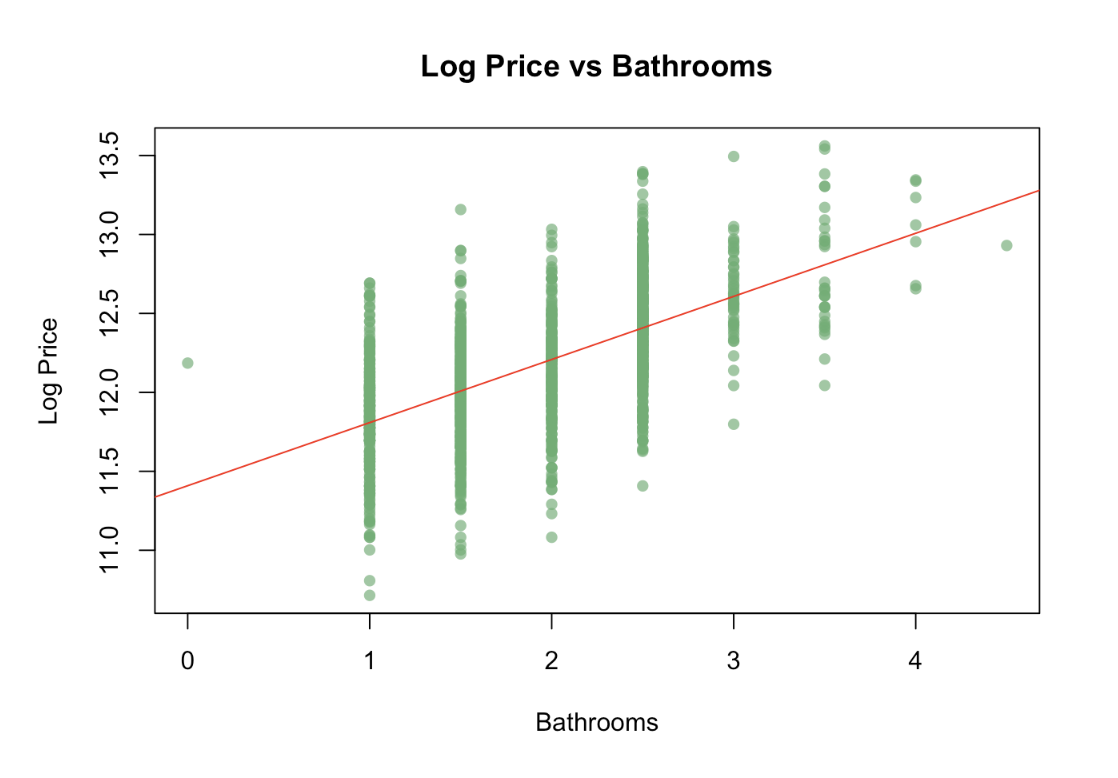
\includegraphics[width=0.43\textwidth,height=\textheight]{A1 Bathrooms.png}

\subsection{Appendix 2}\label{appendix-2}

\begin{table}[H]
\centering
\begin{tabular}{|c|c|}
\hline
\textbf{Predictor} & \textbf{VIF Value} \\
\hline
log\_age & 1.249816 \\
living\_area & 3.181138 \\
bathrooms & 2.287007 \\
rooms & 2.109127 \\
\hline
\end{tabular}
\end{table}

\subsection{Appendix 3}\label{appendix-3}

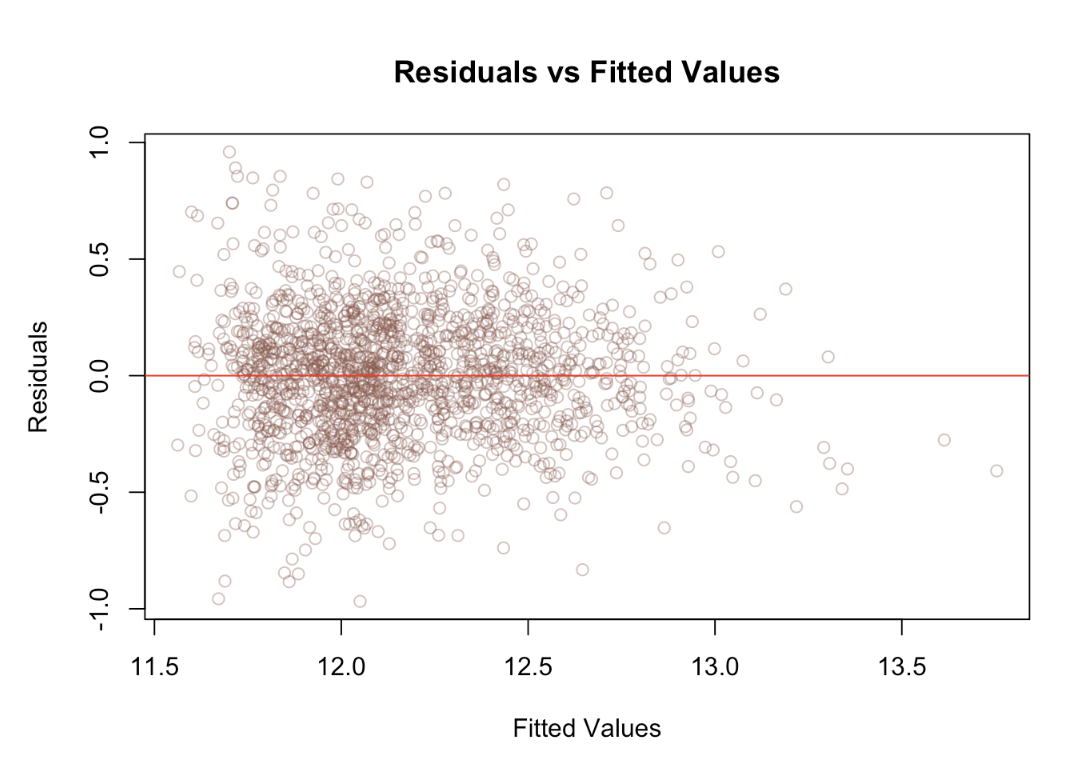
\includegraphics[width=0.45\textwidth,height=\textheight]{A3 Residuals.png}

\subsection{Appendix 4}\label{appendix-4}

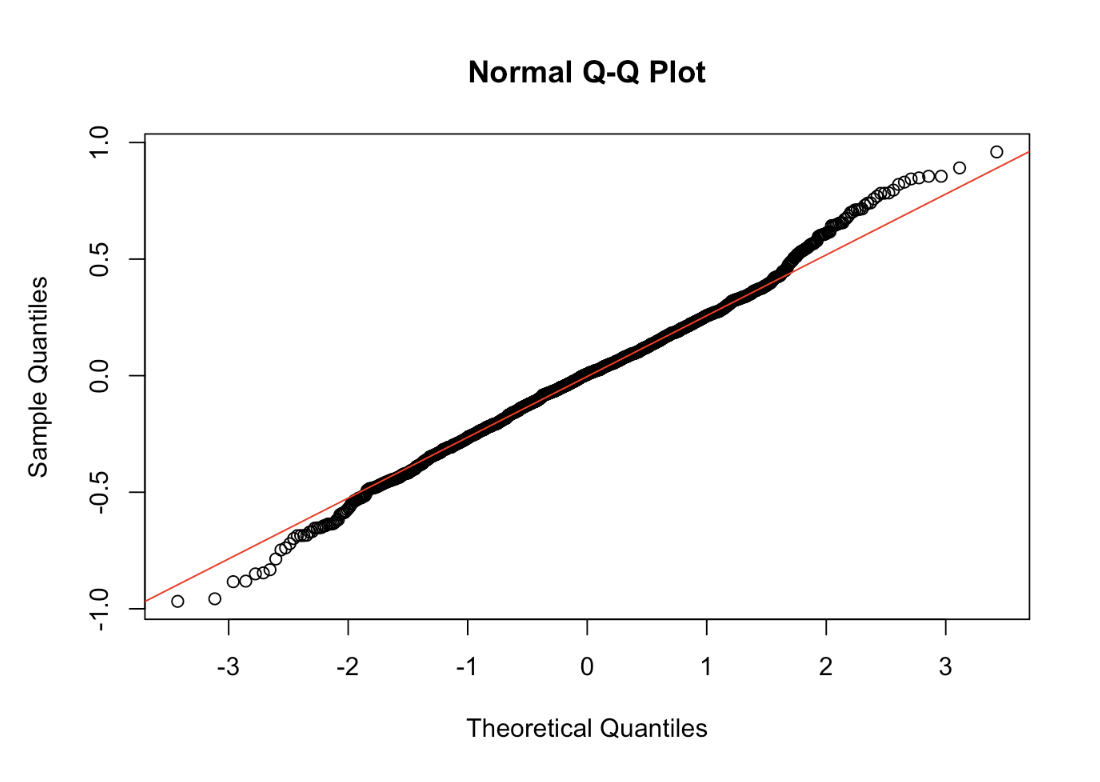
\includegraphics[width=0.5\textwidth,height=\textheight]{A4 QQ-plot.png}

\subsection{References}\label{references}

\begin{enumerate}
\def\labelenumi{\arabic{enumi}.}
\item
  \textbf{Quarto Documentation.} (2024). \emph{PDF Basics.} Retrieved
  from
  \url{https://quarto.org/docs/output-formats/pdf-basics.html\#latex-output}.
\item
  \textbf{Quarto Documentation.} (2024). \emph{Article Layout.}
  Retrieved from
  \url{https://quarto.org/docs/authoring/article-layout.html\#pdflatex-layout}.
\end{enumerate}



\end{document}
